\documentclass{standalone}
\usepackage{tikz}
\usetikzlibrary{patterns, positioning}


\begin{document}
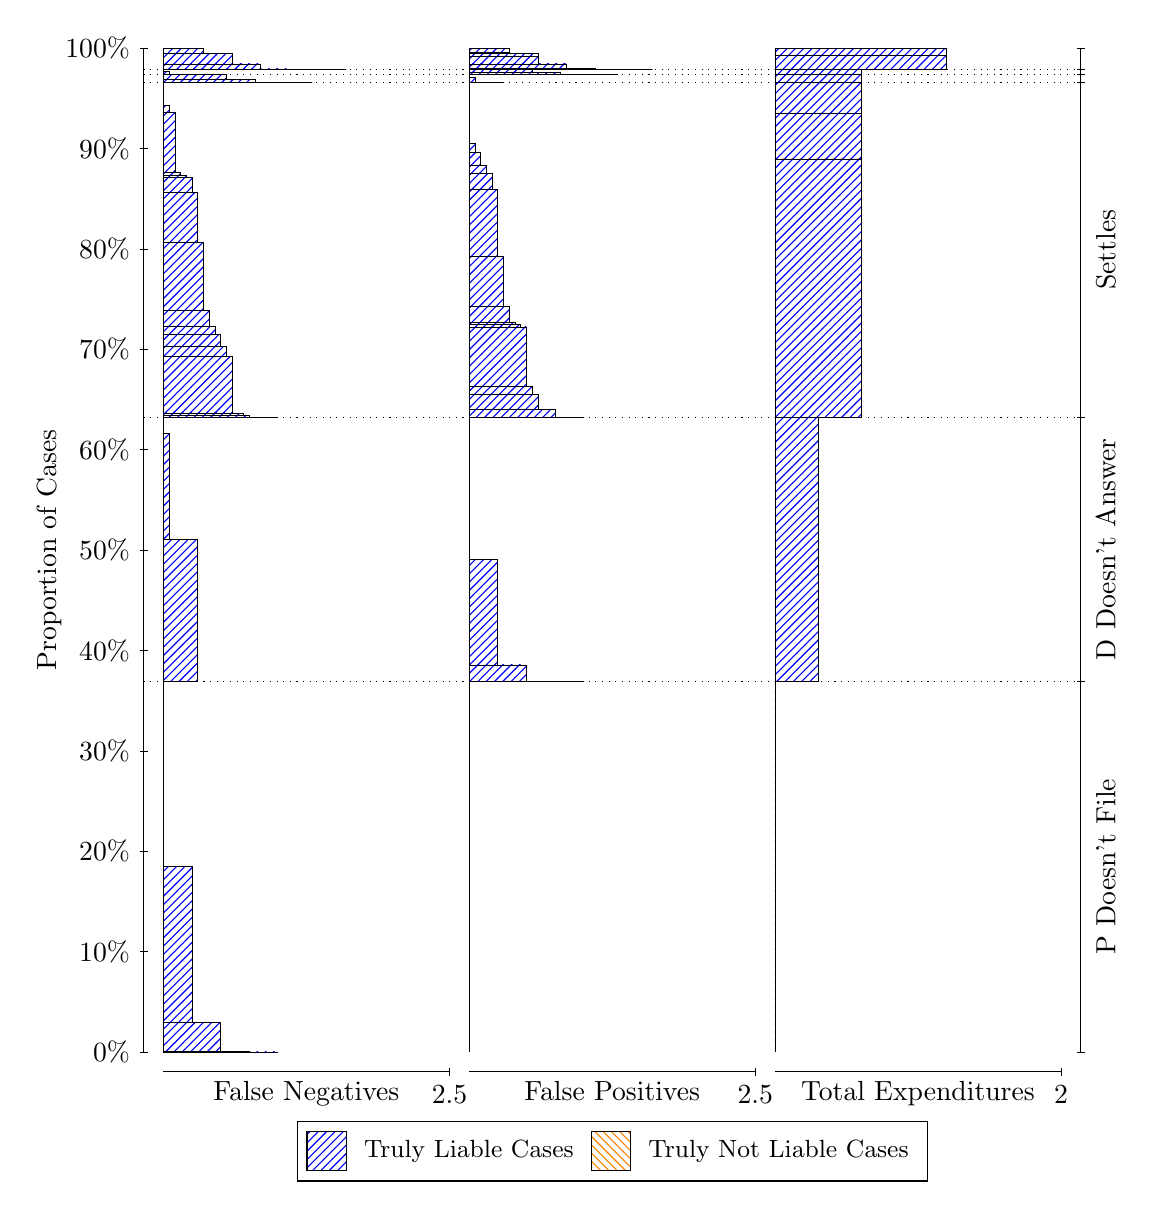
\begin{tikzpicture}
\draw[black, very thin] (1.5,1.75) -- (1.5,14.5);
\node[rotate=90, text=black, anchor=center] at (0.3, 8.125) {Proportion of Cases};
\draw[black, very thin] (1.45,1.75) -- (1.55,1.75);
\node[text=black, anchor=east] at (1.45, 1.75) {0\%};
\draw[black, very thin] (1.45,3.025) -- (1.55,3.025);
\node[text=black, anchor=east] at (1.45, 3.025) {10\%};
\draw[black, very thin] (1.45,4.3) -- (1.55,4.3);
\node[text=black, anchor=east] at (1.45, 4.3) {20\%};
\draw[black, very thin] (1.45,5.575) -- (1.55,5.575);
\node[text=black, anchor=east] at (1.45, 5.575) {30\%};
\draw[black, very thin] (1.45,6.85) -- (1.55,6.85);
\node[text=black, anchor=east] at (1.45, 6.85) {40\%};
\draw[black, very thin] (1.45,8.125) -- (1.55,8.125);
\node[text=black, anchor=east] at (1.45, 8.125) {50\%};
\draw[black, very thin] (1.45,9.4) -- (1.55,9.4);
\node[text=black, anchor=east] at (1.45, 9.4) {60\%};
\draw[black, very thin] (1.45,10.675) -- (1.55,10.675);
\node[text=black, anchor=east] at (1.45, 10.675) {70\%};
\draw[black, very thin] (1.45,11.95) -- (1.55,11.95);
\node[text=black, anchor=east] at (1.45, 11.95) {80\%};
\draw[black, very thin] (1.45,13.225) -- (1.55,13.225);
\node[text=black, anchor=east] at (1.45, 13.225) {90\%};
\draw[black, very thin] (1.45,14.5) -- (1.55,14.5);
\node[text=black, anchor=east] at (1.45, 14.5) {100\%};

\draw[black, very thin] (13.4,1.75) -- (13.4,14.5);
\draw[black, very thin] (13.35,1.75) -- (13.45,1.75);
\node[anchor=west] at (13.35, 1.75) {};
\draw[black, very thin] (13.35,6.4566) -- (13.45,6.4566);
\node[anchor=west] at (13.35, 6.4566) {};
\draw[black, very thin] (13.35,9.813) -- (13.45,9.813);
\node[anchor=west] at (13.35, 9.813) {};
\draw[black, very thin] (13.35,14.066) -- (13.45,14.066);
\node[anchor=west] at (13.35, 14.066) {};
\draw[black, very thin] (13.35,14.165) -- (13.45,14.165);
\node[anchor=west] at (13.35, 14.165) {};
\draw[black, very thin] (13.35,14.232) -- (13.45,14.232);
\node[anchor=west] at (13.35, 14.232) {};
\draw[black, very thin] (13.35,14.5) -- (13.45,14.5);
\node[anchor=west] at (13.35, 14.5) {};

\draw[black, very thin, pattern color=blue, pattern=north east lines] (1.75,1.75) rectangle (3.2033,1.75);
\draw[black, very thin, pattern color=blue, pattern=north east lines] (1.75,1.75) rectangle (2.84,1.7532);
\draw[black, very thin, pattern color=blue, pattern=north east lines] (1.75,1.7532) rectangle (2.4767,2.1267);
\draw[black, very thin, pattern color=blue, pattern=north east lines] (1.75,2.1267) rectangle (2.1133,4.1066);
\draw[black, very thin, pattern color=orange, pattern=north west lines] (1.75,4.1066) rectangle (1.75,4.1066);
\draw[black, very thin, pattern color=blue, pattern=north east lines] (1.75,4.1066) rectangle (1.75,6.4566);
\draw[black, very thin, pattern color=blue, pattern=north east lines] (1.75,6.4566) rectangle (2.186,8.2625);
\draw[black, very thin, pattern color=blue, pattern=north east lines] (1.75,8.2625) rectangle (1.8227,9.6027);
\draw[black, very thin, pattern color=orange, pattern=north west lines] (1.75,9.6027) rectangle (1.75,9.6027);
\draw[black, very thin, pattern color=blue, pattern=north east lines] (1.75,9.6027) rectangle (1.75,9.813);
\draw[black, very thin, pattern color=blue, pattern=north east lines] (1.75,9.813) rectangle (3.2033,9.813);
\draw[black, very thin, pattern color=blue, pattern=north east lines] (1.75,9.813) rectangle (3.058,9.813);
\draw[black, very thin, pattern color=blue, pattern=north east lines] (1.75,9.813) rectangle (2.9127,9.8133);
\draw[black, very thin, pattern color=blue, pattern=north east lines] (1.75,9.8133) rectangle (2.84,9.8322);
\draw[black, very thin, pattern color=blue, pattern=north east lines] (1.75,9.8322) rectangle (2.7673,9.8566);
\draw[black, very thin, pattern color=blue, pattern=north east lines] (1.75,9.8566) rectangle (2.6947,9.8664);
\draw[black, very thin, pattern color=blue, pattern=north east lines] (1.75,9.8664) rectangle (2.622,10.584);
\draw[black, very thin, pattern color=blue, pattern=north east lines] (1.75,10.584) rectangle (2.5493,10.706);
\draw[black, very thin, pattern color=blue, pattern=north east lines] (1.75,10.706) rectangle (2.4767,10.867);
\draw[black, very thin, pattern color=blue, pattern=north east lines] (1.75,10.867) rectangle (2.404,10.967);
\draw[black, very thin, pattern color=blue, pattern=north east lines] (1.75,10.967) rectangle (2.3313,11.171);
\draw[black, very thin, pattern color=blue, pattern=north east lines] (1.75,11.171) rectangle (2.2587,12.028);
\draw[black, very thin, pattern color=blue, pattern=north east lines] (1.75,12.028) rectangle (2.186,12.662);
\draw[black, very thin, pattern color=blue, pattern=north east lines] (1.75,12.662) rectangle (2.1133,12.86);
\draw[black, very thin, pattern color=blue, pattern=north east lines] (1.75,12.86) rectangle (2.0407,12.884);
\draw[black, very thin, pattern color=blue, pattern=north east lines] (1.75,12.884) rectangle (1.968,12.92);
\draw[black, very thin, pattern color=blue, pattern=north east lines] (1.75,12.92) rectangle (1.8953,13.68);
\draw[black, very thin, pattern color=blue, pattern=north east lines] (1.75,13.68) rectangle (1.8227,13.774);
\draw[black, very thin, pattern color=orange, pattern=north west lines] (1.75,13.774) rectangle (1.75,13.774);
\draw[black, very thin, pattern color=blue, pattern=north east lines] (1.75,13.774) rectangle (1.75,14.066);
\draw[black, very thin, pattern color=blue, pattern=north east lines] (1.75,14.066) rectangle (3.6393,14.066);
\draw[black, very thin, pattern color=blue, pattern=north east lines] (1.75,14.066) rectangle (3.276,14.066);
\draw[black, very thin, pattern color=blue, pattern=north east lines] (1.75,14.066) rectangle (2.9127,14.103);
\draw[black, very thin, pattern color=blue, pattern=north east lines] (1.75,14.103) rectangle (2.5493,14.164);
\draw[black, very thin, pattern color=blue, pattern=north east lines] (1.75,14.164) rectangle (2.186,14.165);
\draw[black, very thin, pattern color=orange, pattern=north west lines] (1.75,14.165) rectangle (1.75,14.165);
\draw[black, very thin, pattern color=blue, pattern=north east lines] (1.75,14.165) rectangle (2.186,14.166);
\draw[black, very thin, pattern color=blue, pattern=north east lines] (1.75,14.166) rectangle (1.8227,14.207);
\draw[black, very thin, pattern color=orange, pattern=north west lines] (1.75,14.207) rectangle (1.75,14.207);
\draw[black, very thin, pattern color=blue, pattern=north east lines] (1.75,14.207) rectangle (1.75,14.232);
\draw[black, very thin, pattern color=blue, pattern=north east lines] (1.75,14.232) rectangle (4.0753,14.232);
\draw[black, very thin, pattern color=blue, pattern=north east lines] (1.75,14.232) rectangle (3.712,14.232);
\draw[black, very thin, pattern color=blue, pattern=north east lines] (1.75,14.232) rectangle (3.3487,14.236);
\draw[black, very thin, pattern color=blue, pattern=north east lines] (1.75,14.236) rectangle (2.9853,14.298);
\draw[black, very thin, pattern color=blue, pattern=north east lines] (1.75,14.298) rectangle (2.622,14.433);
\draw[black, very thin, pattern color=blue, pattern=north east lines] (1.75,14.433) rectangle (2.2587,14.495);
\draw[black, very thin, pattern color=blue, pattern=north east lines] (1.75,14.495) rectangle (1.8953,14.5);
\draw[black, very thin, pattern color=orange, pattern=north west lines] (1.75,14.5) rectangle (1.75,14.5);
\draw[black, very thin, pattern color=blue, pattern=north east lines] (1.75,14.5) rectangle (1.75,14.5);
\draw[black, very thin, pattern color=orange, pattern=north west lines] (5.6333,1.75) rectangle (5.6333,1.75);
\draw[black, very thin, pattern color=blue, pattern=north east lines] (5.6333,1.75) rectangle (5.6333,6.4566);
\draw[black, very thin, pattern color=orange, pattern=north west lines] (5.6333,6.4566) rectangle (7.0867,6.4566);
\draw[black, very thin, pattern color=blue, pattern=north east lines] (5.6333,6.4566) rectangle (7.0867,6.4566);
\draw[black, very thin, pattern color=blue, pattern=north east lines] (5.6333,6.4566) rectangle (6.7233,6.4572);
\draw[black, very thin, pattern color=blue, pattern=north east lines] (5.6333,6.4572) rectangle (6.36,6.6669);
\draw[black, very thin, pattern color=blue, pattern=north east lines] (5.6333,6.6669) rectangle (5.9967,8.0071);
\draw[black, very thin, pattern color=blue, pattern=north east lines] (5.6333,8.0071) rectangle (5.6333,9.813);
\draw[black, very thin, pattern color=orange, pattern=north west lines] (5.6333,9.813) rectangle (7.0867,9.813);
\draw[black, very thin, pattern color=blue, pattern=north east lines] (5.6333,9.813) rectangle (7.0867,9.8132);
\draw[black, very thin, pattern color=orange, pattern=north west lines] (5.6333,9.8132) rectangle (6.9413,9.8132);
\draw[black, very thin, pattern color=blue, pattern=north east lines] (5.6333,9.8132) rectangle (6.9413,9.8132);
\draw[black, very thin, pattern color=orange, pattern=north west lines] (5.6333,9.8132) rectangle (6.796,9.8132);
\draw[black, very thin, pattern color=blue, pattern=north east lines] (5.6333,9.8132) rectangle (6.796,9.8134);
\draw[black, very thin, pattern color=blue, pattern=north east lines] (5.6333,9.8134) rectangle (6.7233,9.9082);
\draw[black, very thin, pattern color=orange, pattern=north west lines] (5.6333,9.9082) rectangle (6.6507,9.9082);
\draw[black, very thin, pattern color=blue, pattern=north east lines] (5.6333,9.9082) rectangle (6.6507,9.9085);
\draw[black, very thin, pattern color=blue, pattern=north east lines] (5.6333,9.9085) rectangle (6.578,9.9085);
\draw[black, very thin, pattern color=orange, pattern=north west lines] (5.6333,9.9085) rectangle (6.5053,9.9085);
\draw[black, very thin, pattern color=blue, pattern=north east lines] (5.6333,9.9085) rectangle (6.5053,10.104);
\draw[black, very thin, pattern color=blue, pattern=north east lines] (5.6333,10.104) rectangle (6.4327,10.199);
\draw[black, very thin, pattern color=blue, pattern=north east lines] (5.6333,10.199) rectangle (6.36,10.959);
\draw[black, very thin, pattern color=blue, pattern=north east lines] (5.6333,10.959) rectangle (6.2873,10.994);
\draw[black, very thin, pattern color=blue, pattern=north east lines] (5.6333,10.994) rectangle (6.2147,11.019);
\draw[black, very thin, pattern color=blue, pattern=north east lines] (5.6333,11.019) rectangle (6.142,11.216);
\draw[black, very thin, pattern color=blue, pattern=north east lines] (5.6333,11.216) rectangle (6.0693,11.85);
\draw[black, very thin, pattern color=blue, pattern=north east lines] (5.6333,11.85) rectangle (5.9967,12.707);
\draw[black, very thin, pattern color=blue, pattern=north east lines] (5.6333,12.707) rectangle (5.924,12.912);
\draw[black, very thin, pattern color=blue, pattern=north east lines] (5.6333,12.912) rectangle (5.8513,13.012);
\draw[black, very thin, pattern color=blue, pattern=north east lines] (5.6333,13.012) rectangle (5.7787,13.173);
\draw[black, very thin, pattern color=blue, pattern=north east lines] (5.6333,13.173) rectangle (5.706,13.295);
\draw[black, very thin, pattern color=blue, pattern=north east lines] (5.6333,13.295) rectangle (5.6333,14.066);
\draw[black, very thin, pattern color=orange, pattern=north west lines] (5.6333,14.066) rectangle (6.0693,14.066);
\draw[black, very thin, pattern color=blue, pattern=north east lines] (5.6333,14.066) rectangle (6.0693,14.067);
\draw[black, very thin, pattern color=blue, pattern=north east lines] (5.6333,14.067) rectangle (5.706,14.128);
\draw[black, very thin, pattern color=blue, pattern=north east lines] (5.6333,14.128) rectangle (5.6333,14.165);
\draw[black, very thin, pattern color=orange, pattern=north west lines] (5.6333,14.165) rectangle (7.5227,14.165);
\draw[black, very thin, pattern color=blue, pattern=north east lines] (5.6333,14.165) rectangle (7.5227,14.165);
\draw[black, very thin, pattern color=blue, pattern=north east lines] (5.6333,14.165) rectangle (7.1593,14.165);
\draw[black, very thin, pattern color=blue, pattern=north east lines] (5.6333,14.165) rectangle (6.796,14.19);
\draw[black, very thin, pattern color=blue, pattern=north east lines] (5.6333,14.19) rectangle (6.4327,14.231);
\draw[black, very thin, pattern color=blue, pattern=north east lines] (5.6333,14.231) rectangle (6.0693,14.232);
\draw[black, very thin, pattern color=orange, pattern=north west lines] (5.6333,14.232) rectangle (7.9587,14.232);
\draw[black, very thin, pattern color=blue, pattern=north east lines] (5.6333,14.232) rectangle (7.9587,14.232);
\draw[black, very thin, pattern color=orange, pattern=north west lines] (5.6333,14.232) rectangle (7.5953,14.232);
\draw[black, very thin, pattern color=blue, pattern=north east lines] (5.6333,14.232) rectangle (7.5953,14.232);
\draw[black, very thin, pattern color=orange, pattern=north west lines] (5.6333,14.232) rectangle (7.232,14.232);
\draw[black, very thin, pattern color=blue, pattern=north east lines] (5.6333,14.232) rectangle (7.232,14.237);
\draw[black, very thin, pattern color=blue, pattern=north east lines] (5.6333,14.237) rectangle (6.8687,14.298);
\draw[black, very thin, pattern color=orange, pattern=north west lines] (5.6333,14.298) rectangle (6.8687,14.298);
\draw[black, very thin, pattern color=blue, pattern=north east lines] (5.6333,14.298) rectangle (6.8687,14.299);
\draw[black, very thin, pattern color=blue, pattern=north east lines] (5.6333,14.299) rectangle (6.5053,14.389);
\draw[black, very thin, pattern color=orange, pattern=north west lines] (5.6333,14.389) rectangle (6.5053,14.389);
\draw[black, very thin, pattern color=blue, pattern=north east lines] (5.6333,14.389) rectangle (6.5053,14.434);
\draw[black, very thin, pattern color=blue, pattern=north east lines] (5.6333,14.434) rectangle (6.142,14.448);
\draw[black, very thin, pattern color=blue, pattern=north east lines] (5.6333,14.448) rectangle (6.142,14.496);
\draw[black, very thin, pattern color=blue, pattern=north east lines] (5.6333,14.496) rectangle (5.7787,14.496);
\draw[black, very thin, pattern color=blue, pattern=north east lines] (5.6333,14.496) rectangle (5.7787,14.5);
\draw[black, very thin, pattern color=blue, pattern=north east lines] (5.6333,14.5) rectangle (5.6333,14.5);
\draw[black, very thin, pattern color=orange, pattern=north west lines] (9.5167,1.75) rectangle (9.5167,1.75);
\draw[black, very thin, pattern color=blue, pattern=north east lines] (9.5167,1.75) rectangle (9.5167,6.4566);
\draw[black, very thin, pattern color=orange, pattern=north west lines] (9.5167,6.4566) rectangle (10.062,6.4566);
\draw[black, very thin, pattern color=blue, pattern=north east lines] (9.5167,6.4566) rectangle (10.062,9.813);
\draw[black, very thin, pattern color=orange, pattern=north west lines] (9.5167,9.813) rectangle (10.607,9.813);
\draw[black, very thin, pattern color=blue, pattern=north east lines] (9.5167,9.813) rectangle (10.607,13.093);
\draw[black, very thin, pattern color=orange, pattern=north west lines] (9.5167,13.093) rectangle (10.607,13.093);
\draw[black, very thin, pattern color=blue, pattern=north east lines] (9.5167,13.093) rectangle (10.607,13.667);
\draw[black, very thin, pattern color=orange, pattern=north west lines] (9.5167,13.667) rectangle (10.607,13.667);
\draw[black, very thin, pattern color=blue, pattern=north east lines] (9.5167,13.667) rectangle (10.607,14.066);
\draw[black, very thin, pattern color=orange, pattern=north west lines] (9.5167,14.066) rectangle (10.607,14.066);
\draw[black, very thin, pattern color=blue, pattern=north east lines] (9.5167,14.066) rectangle (10.607,14.165);
\draw[black, very thin, pattern color=orange, pattern=north west lines] (9.5167,14.165) rectangle (10.607,14.165);
\draw[black, very thin, pattern color=blue, pattern=north east lines] (9.5167,14.165) rectangle (10.607,14.232);
\draw[black, very thin, pattern color=orange, pattern=north west lines] (9.5167,14.232) rectangle (11.697,14.232);
\draw[black, very thin, pattern color=blue, pattern=north east lines] (9.5167,14.232) rectangle (11.697,14.402);
\draw[black, very thin, pattern color=orange, pattern=north west lines] (9.5167,14.402) rectangle (11.697,14.402);
\draw[black, very thin, pattern color=blue, pattern=north east lines] (9.5167,14.402) rectangle (11.697,14.5);
\draw[black, dotted] (1.5,6.4566) -- (13.4,6.4566);
\draw[black, dotted] (1.5,9.813) -- (13.4,9.813);
\draw[black, dotted] (1.5,14.066) -- (13.4,14.066);
\draw[black, dotted] (1.5,14.165) -- (13.4,14.165);
\draw[black, dotted] (1.5,14.232) -- (13.4,14.232);
\draw[black, very thin] (1.75,1.5) -- (5.3833,1.5);
\node[text=black, anchor=north] at (3.5667, 1.5) {False Negatives};
\draw[black, very thin] (5.3833,1.45) -- (5.3833,1.55);
\node[text=black, anchor=north] at (5.3833, 1.45) {2.5};

\draw[black, very thin] (5.6333,1.5) -- (9.2667,1.5);
\node[text=black, anchor=north] at (7.45, 1.5) {False Positives};
\draw[black, very thin] (9.2667,1.45) -- (9.2667,1.55);
\node[text=black, anchor=north] at (9.2667, 1.45) {2.5};

\draw[black, very thin] (9.5167,1.5) -- (13.15,1.5);
\node[text=black, anchor=north] at (11.333, 1.5) {Total Expenditures};
\draw[black, very thin] (13.15,1.45) -- (13.15,1.55);
\node[text=black, anchor=north] at (13.15, 1.45) {2};

\node[text=black, centered, rotate=90] at (13.72, 4.1033) {P Doesn't File};
\node[text=black, centered, rotate=90] at (13.72, 8.1348) {D Doesn't Answer};
\node[text=black, centered, rotate=90] at (13.72, 11.939) {Settles};




\draw (7.449999999999999,1.5) node[draw=none] (baseCoordinate) {};
\begin{scope}[align=center]
        \matrix[scale=0.5, draw=black, below=0.5cm of baseCoordinate, nodes={draw}, column sep=0.1cm]{
            \node[rectangle, draw, minimum width=0.5cm, minimum height=0.5cm, pattern color=blue, pattern=north east lines] {}; &
            \node[draw=none, font=\small, text=black] (B) {Truly Liable Cases}; &
            \node[rectangle, draw, minimum width=0.5cm, minimum height=0.5cm, pattern color=orange, pattern=north west lines] {}; &
            \node[draw=none, font=\small, text=black] (B) {Truly Not Liable Cases}; \\
            };
\end{scope}

\end{tikzpicture}
\end{document}